\documentclass[aps,reprint]{revtex4-1}
% Engine-specific settings
% Detect pdftex/xetex/luatex, and load appropriate font packages.
% This is inspired by the approach in the iftex package.
% pdftex:
\ifx\pdfmatch\undefined
\else
    \usepackage[T1]{fontenc}
    \usepackage[utf8]{inputenc}
\fi
% xetex:
\ifx\XeTeXinterchartoks\undefined
\else
    \usepackage{fontspec}
    \defaultfontfeatures{Ligatures=TeX}
\fi
% luatex:
\ifx\directlua\undefined
\else
    \usepackage{fontspec}
\fi
% End engine-specific settings
\usepackage[norsk]{babel}
\usepackage{csquotes}
% \usepackage[backend=biber, sortcites]{biblatex}
\usepackage{url}
\usepackage{textcomp}
\usepackage[usenames,dvipsnames,svgnames, table]{xcolor}
\usepackage[font={scriptsize}]{caption}
\usepackage{amsmath} \usepackage{amsthm} \usepackage{amsfonts}
\usepackage{amssymb}
\usepackage{enumerate}
\usepackage{tikz} \usepackage{float}
\usepackage[procnames]{listings}
\usepackage{pstool} \usepackage{pgfplots}
\usepackage{wrapfig} \usepackage{graphicx} \usepackage{epstopdf}
\usepackage{afterpage}
\usepackage{physics}
\usepackage{multirow}
\usepackage{gensymb}
\usepackage{algorithm}
\usepackage{microtype}
\usepackage[noend]{algpseudocode}
\usepackage{xcolor,colortbl}
\usepackage{microtype}
\usepackage{geometry}
\usepackage{hyperref}
\usepackage{graphicx}
\usepackage{caption}
\usepackage{subcaption}
\usepackage{lipsum}
% \usepackage{pythontex}
% \usepackage{authblk}
\usepackage{nth}
\usepackage{siunitx}
% \usepackage[toc,page]{appendix}
\floatstyle{plaintop}
\restylefloat{table}

% Custom commands
\newcommand{\unit}[1]{\:\mathrm{#1}}
\newcommand{\noref}[1]{\hyperref[#1]{\ref*{#1}}}
\newcommand{\nonref}[1]{\hyperref[]{\ref*{#1}}}
\newcommand\blankpage{%
  \null
  \thispagestyle{empty}%
  \addtocounter{page}{-1}%
  \newpage}

% Default fixed font does not support bold face
\DeclareFixedFont{\ttb}{T1}{txtt}{bx}{n}{7} % for bold
\DeclareFixedFont{\ttm}{T1}{txtt}{m}{n}{7}  % for normal

\newcommand\numberthis{\addtocounter{equation}{1}\tag{\theequation}}

% Biber for references
% \bibliographystyle{aipauth4-1}

\begin{document}
\sisetup{detect-all}
\title{Faseoverganger - Laboratorieøvelse 1 FYS2160}
\author{V. Mäntysalo}
\author{M. Nilsen}
\author{F. Mellbye}
\affiliation{Universitetet i Oslo, Oslo, Norge}
\date{\today}

\begin{abstract}
Smeltevarmen for is og fordampningsvarmen til vann ved 100 C blir bestemt, med trykket i begge tilfeller lik atmosfæretrykket.
\end{abstract}
\maketitle
\makeatletter
\let\toc@pre\relax
\let\toc@post\relax
\makeatother
\section{Smeltevarmen for is}
\subsection{Teori}
Den spesifikke smeltevarmen for is er den energien som trengs for å omdanne
$1$ kg (ett mol) is med temperatur $0 \degree$ C til vann med temperatur $0\degree$ C.
\subsection{Metode}
\subsubsection{Apparatur}
Følgende utstyr ble benyttet til å bestemme smeltevarmen til is:
\begin{itemize}
  \item Kalorimeter
  \item Strømforsyning
  \item Amperemeter
  \item Voltmeter
  \item Termometer (PASCO, koblet til PC via USB)
  \item Digitalvekt
  \item Isblokk i et isvannbad (kar med is og vann)
\end{itemize}
Kalorimeteret består av en isoporisolert beholder av rustfritt stål med et plastlokk
som er påmontert et varmeelement og en rører. Termometerets føler ble ført ned
i kalorimeteret gjennom et hull i lokket.
\subsubsection{Utførelse}
\noindent
Fullstendig utførelse finnes i REF. Varmekapasiteten $C_0$ til hele kalorimeteret
med innhold beregnes ved hjelp av ligningen
\begin{align}
  \label{eq:varmekapasitet}
  C_0 \frac{\text{d} T}{\text{d} t} = U \cdot I
\end{align}
der $I$ er strømmen gjennom og $U$ er potensialet over varmelementet. Når denne
verdien er funnet for oppsettet blir eksperimentet utført ved å smelte en isklump
i kalorimeteret mens temperaturen logges.
\begin{figure}[H]
  \centering
  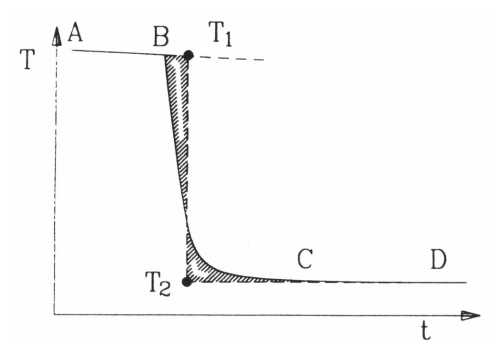
\includegraphics[width=\linewidth]{tempforlop.png}
  \caption{Temperaturforløpet i kalorimeteret}
  \label{fig:tempforlop}
\end{figure}
\subsubsection{Beregning av smeltevarmen}
\noindent
Den spesifikke smeltevarmen $L_S$ beregnes med
\begin{align*}
  m[L_S + C_v (T_2 - T_0)] = C_0 (T_1 - T_2)
\end{align*}
som løst for $L_S$ sier at
\begin{align}
  \label{eq:smeltevarmeligning}
  L_S = \frac{C_0 (T_1 - T_2)}{m} - C_v (T_2 - T_0)
\end{align}
\noindent
(\textbf{Oppgave 3 - Tolkning av formel ~\ref{eq:smeltevarmeligning}:})
$L_s$ angir den spesifikke smeltevarmen, som er mengden energi som kreves
per enhets masse for å omdanne et stoff fra fast stoff til væskefase (smelting).
Ligning ~\ref{eq:smeltevarmeligning} er en energibevaringsligning for
systemet med isblokken satt inn. Det første leddet er energien bundet til
smelting av isblokken, det andre leddet omhandler den termiske energien til
mediet isblokken er lagt ned i (vannet), og dette er lik kalorimeterets
(systemets) totale energi.
\subsection{Resultater}
\subsubsection{Bestemmelse av varmekapasiteten til kalorimeteret}
Avlesning fra apparatene under oppvarmingen gir
\begin{align*}
  I &= (0.7545 \pm 0.001) \text{A} \\
  V &= (88.920 \pm 0.020) \text{V}
\end{align*}
der usikkerhetene er omtrentlige fra avlesningen fra apparatene (verdiene
svingte tilfeldig innenfor intervallene over.) Fra Capstone avleses stigningstallet $\text{d}T/\text{d}t$
med lineærtilpasning (se vedlegg)
\begin{align*}
  \frac{\text{d}T}{\text{d}t} = 0.0116 \pm 1.7 \cdot 10^{-6} \text{J/K}
\end{align*}
Dette gir varmekapasiteten til kalorimeteret som (med ligning ~\ref{eq:varmekapasitet})
\begin{align}
  C_0 \approx 5780.8 \frac{\text{J}}{\text{K}}
\end{align}
\subsubsection{Bestemmelse av smeltevarmen}
\noindent
Isklumpen ble veid til å ha en masse (her er usikkerheten til apparatet ukjent,
og dette kan bidra med en ukjent systematisk feil)
\begin{align*}
  m = 198.98 \text{ g}
\end{align*}
Avlesning fra Capstone (se vedlegg) gir at
\begin{align*}
  T_1 = 30.00 \degree C\\
  T_2 = 15.76 \degree C
\end{align*}
Dette gir at den spesifikke smeltevarmen til is er gitt som
\begin{align}
  L_S = 347.510 \text{ kJ/kg} = 6.246 \text{ kJ/mol}
\end{align}
\section{Fordampningsvarmen for is}
Vi betrakter et system av vann og damp i likevekt ved trykket $P$ og temperaturen
$T$.
\subsection{Teori}
Se oppgavetekst for utfyllende teoretisk introduksjon. Ved antagelsene der og ved hjelp
av Clausius-Clapeyrons ligning kan følgende relasjon utledes:
\begin{align}
  \label{eq:claus}
  \ln{\frac{P_1}{P_2}} = - \frac{L_f}{R}\left( \frac{1}{T_1} - \frac{1}{T_2} \right)
\end{align}
Her er $P_1$ og $P_2$ damptrykkene ved temperaturene $T_1$ og $T_2$, som antas
nær hverandre, og $R = N_A k_B$. Her er $N_A = 6.022 \cdot 10^{23}$ Avogadros
tall og $k_B = 1.3806488 \cdot 10^{-23}$ J/K er Boltzmanns konstant.
\subsection{Metode}
Se figur ~\ref{fig:apparatur} for oppsett.
\begin{figure}[H]
  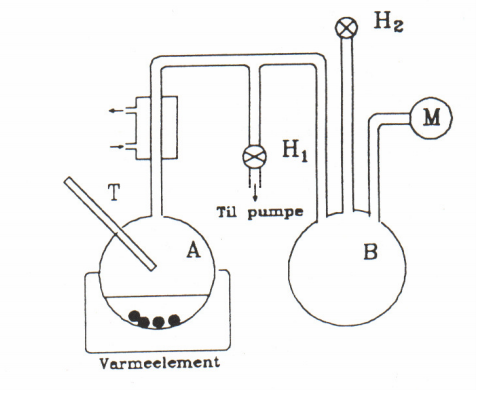
\includegraphics[width = \linewidth]{apparatur.png}
  \caption{Apparatur for måling av damptrykkets temperaturavhengighet.}
  \label{fig:apparatur}
\end{figure}
Kolben A inneholder vann og kokestein som forhindrer støtkoking. Et glassrør
og en slange forbinder kolben med buffervolumet B, som gjør systemet "mykere".
Ved vannstrålepumpen ble systemet redusert fra atomsfæretrykket til rundt
$19$ kPa.
\subsubsection{Utførelse}
Vannstrålepumpen ble startet med hanene lukket. Hanen $H_1$ ble åpnet til trykket
økte med om lag $5$ kPa om gangen, til likevekt oppnås (liten endring i
temperatur med tiden). Denne prosessen ble gjentatt til trykket i kolben
nådde atmosfæretrykk. Verdiene for trykk og temperatur ble avlest med Capstone
for hver likevektstilstand.
\subsection{Resultater}
\subsubsection{Beregning av fordampningsvarmen}
Ifølge lineærtilpasningen i Capstone er stigningstallet til $\ln P$ mot
$T^{-1}$ gitt som
\begin{align*}
  m = -5300 \pm 21
\end{align*}
Dette gir ved ~\ref{eq:claus} at fordampningsvarmen $L_f$ er gitt ved
\begin{align*}
  -\frac{L_f}{R} = -5300
\end{align*}
som gir
\begin{align}
  L_f \approx (44.07 \pm 0.17) \text{kJ/mol}
\end{align}
Ved å kun benytte de tre første datapunktene (hvor antagelsen om $T_1$ og $T_2$ nær hverandre er bedre)
fåes på samme måte at
\begin{align}
  L_f \approx (42.57 \pm 0.7 \text{kJ/mol})
\end{align}
\section{Generell diskusjon (Oppgave 6)}
Kjente verdier for fordampningsvarmen og smeltevarmen er gitt som
\begin{align}
  L_s &= 6.01 \text{ kJ/mol} = 333.55 \text{kJ/kg}\\
  L_f &= 40.66 \text{ kJ/mol}
\end{align}
Til sammenligning er altså de eksperimentelt funnede verdiene gitt ved
\begin{align}
  L_s &= 347.510 \text{ kJ/kg} = 6.246 \text{ kJ/mol} \\
  L_f &= (42.57 \pm 0.7) \text{kJ/mol}
\end{align}
der vi har brukt de tre punktene i fordampningseksperimentet som ligger i
intervallet nærmest antagelsene våre.

Vi ser at begge målingene har gitt litt høyere resultater enn kjente verdier.
Dette skyldes antagelig systematiske feil ved måling, som er vanskelige å estimere.

Vi ser også at fordampningsvarmen er langt høyere enn smeltevarmen. Altså kreves
det langt mer energi å fordampe vann enn å smelte is.

Mulige feilkilder for de systematiske feilene er: At isen smelter noe under
frakt til kalorimeteret, at kalorimeteret mister noe varme ved insertering av
isklumpen, at isklumpen har en inhomogen temperaturfordeling. 
\end{document}

% Local Variables:
% TeX-engine: luatex
% End:
